% To je predloga za poročila o domačih nalogah pri predmetih, katerih
% nosilec je Blaž Zupan. Seveda lahko tudi dodaš kakšen nov, zanimiv
% in uporaben element, ki ga v tej predlogi (še) ni. Več o LaTeX-u izveš na
% spletu, na primer na http://tobi.oetiker.ch/lshort/lshort.pdf.
%
% To predlogo lahko spremeniš v PDF dokument s pomočjo programa
% pdflatex, ki je del standardne instalacije LaTeX programov.

\documentclass[a4paper,11pt]{article}
\usepackage{a4wide}
\usepackage{fullpage}
\usepackage[utf8x]{inputenc}
\usepackage[slovene]{babel}
\selectlanguage{slovene}
\usepackage[toc,page]{appendix}
\usepackage[pdftex]{graphicx} % za slike
\usepackage{setspace}
\usepackage{color}
\definecolor{light-gray}{gray}{0.95}
\usepackage{listings} % za vključevanje kode
\usepackage{hyperref}
\renewcommand{\baselinestretch}{1.2} % za boljšo berljivost večji razmak
\renewcommand{\appendixpagename}{Priloge}

\lstset{ % nastavitve za izpis kode, sem lahko tudi kaj dodaš/spremeniš
language=Python,
basicstyle=\footnotesize,
basicstyle=\ttfamily\footnotesize\setstretch{1},
backgroundcolor=\color{light-gray},
}

\title{%
  Vaja 7\\
  \large Postavitev in upravljanje računalniških oblakov}
\author{David Rubin \\ (david.rubin@student.um.si)}
\date{\today}

\begin{document}

\maketitle

\section{Opis naloge}

Vzpostaviti je bilo potrebno psevdo distribuirano postavitev Hadoop okolja in na njej pognati primer MapReduce programa.

\section{Opis rešitve}

Rešitev sem implementiral v obliki Vagrantfile, ki zažene Ubuntu 18.04 in na njem vzpostavi Hadoop okolje z YARN upravljalcem. Na virtualko se namesti JAVA, zgenerira se nov ključ za povezovanje na \textit{localhost} brez gesla in na virtualko se prenesejo 4 konfiguracijske datoteke: \textit{core-site.xml}, \textit{hdfs-site.xml}, \textit{mapred-site.xml} in \textit{yarn-site.xml}. Za tem se poženejo še ukazi za zagon HDFS in YARN \footnote{Vagrantfile datoteka se nahaja na naslovu \url{https://github.com/rubinda/puro/blob/master/7-hadoop-pseudo/Vagrantfile}}. Za ukaze glej navodila\footnote{Navodila za vzpostavitev psevdo gruče se nahajajo na spletnem naslovu \url{https://hadoop.apache.org/docs/stable/hadoop-project-dist/hadoop-common/SingleCluster.html} }. Na sliki~\ref{namenode} Je prikazan spletni vmesnik Namenode, na sliki~\ref{yarn} je spletni vmesnik Resource managerja (YARN), na sliki ~\ref{example} pa je prikazan izpis po zagonu primera MapReduce programa.


\begin{figure}
\begin{center}
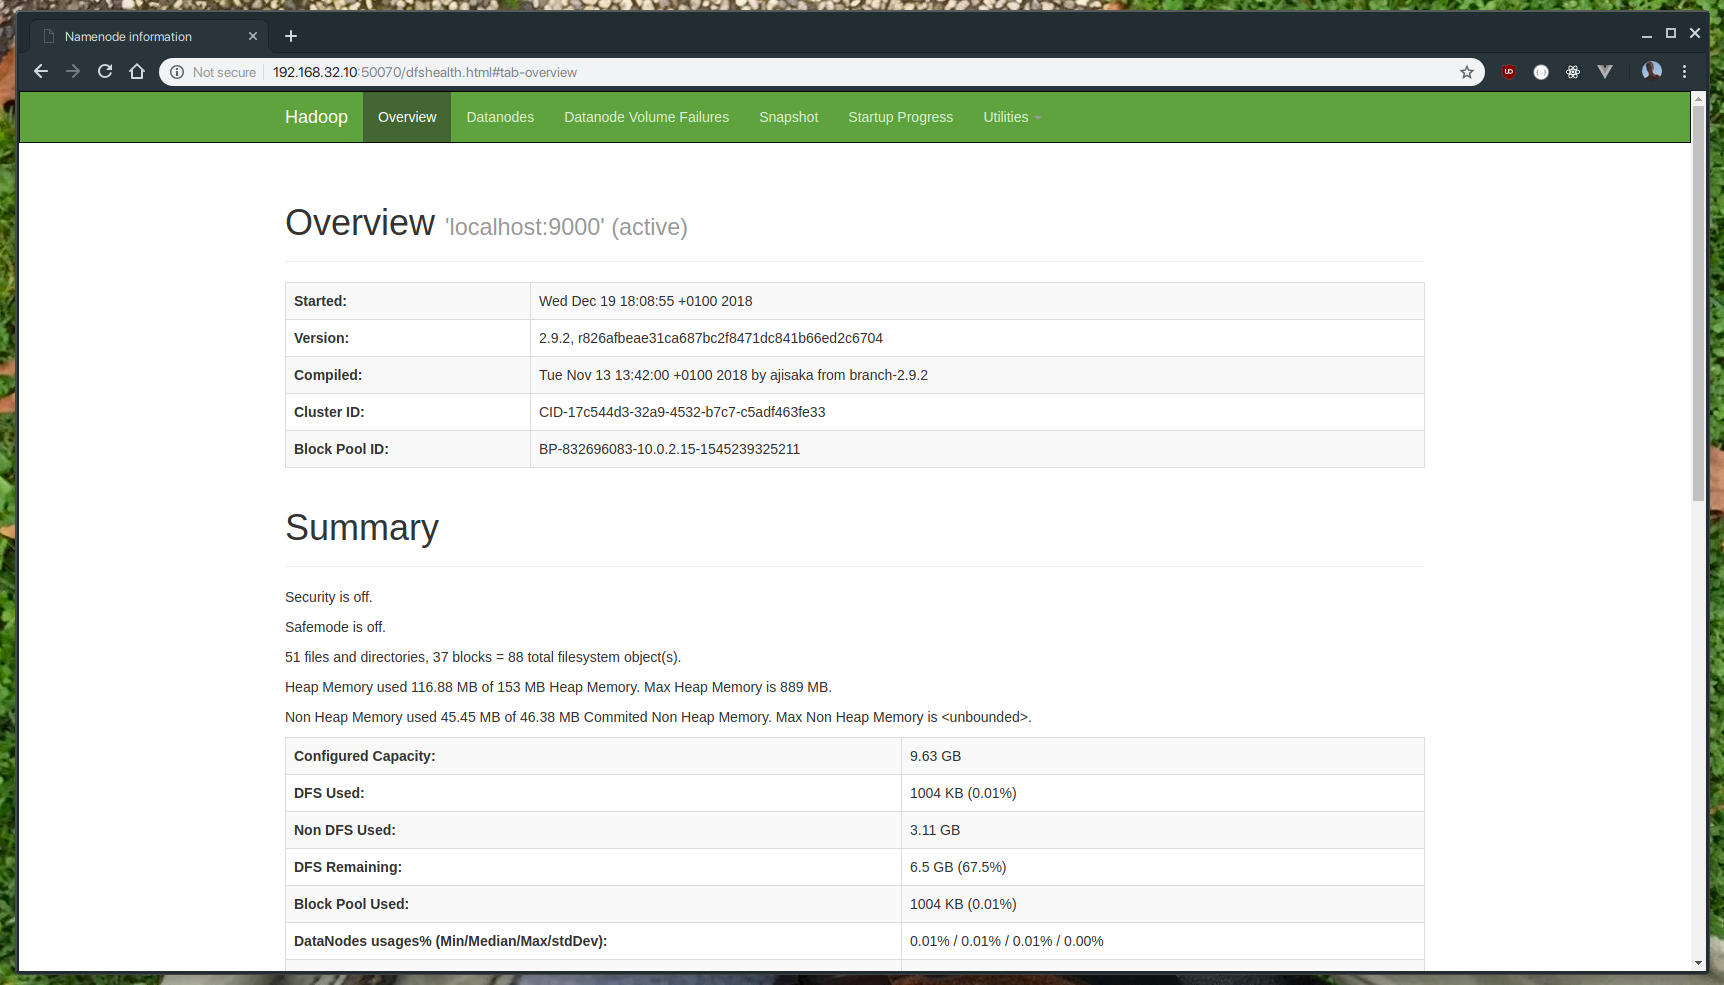
\includegraphics[scale=0.36]{./namenode.png}
\caption{Namenode na vitualki}
\label{namenode}
\end{center}
\end{figure}

\begin{figure}
\begin{center}
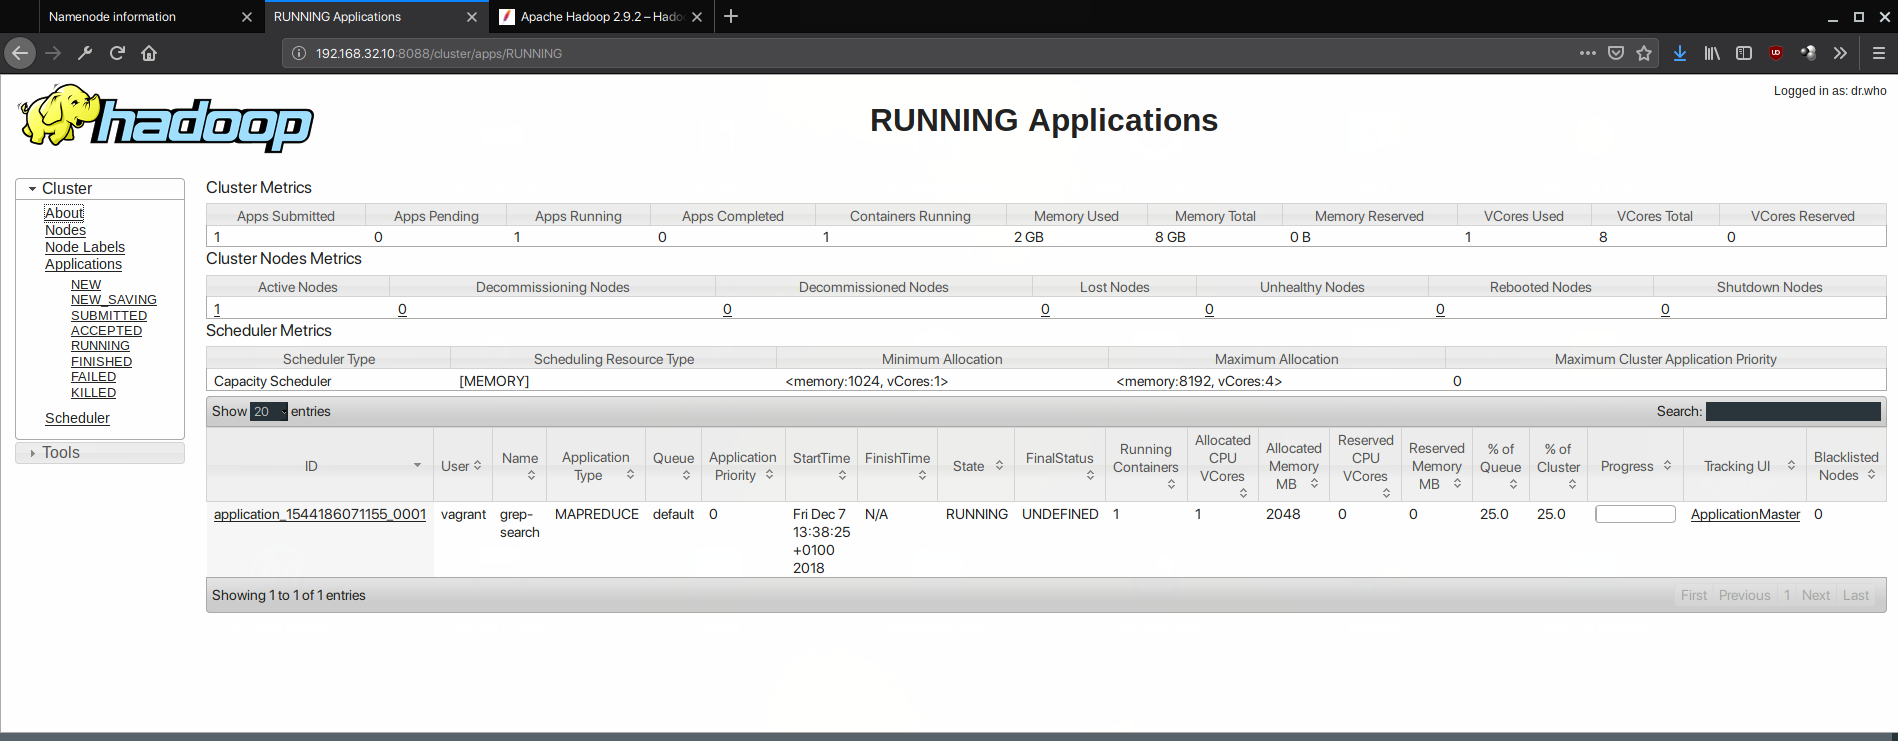
\includegraphics[scale=0.33]{./mapreduce-running.png}
\caption{YARN s tekočim MapReduce opravilom}
\label{yarn}
\end{center}
\end{figure}

\begin{figure}
\begin{center}
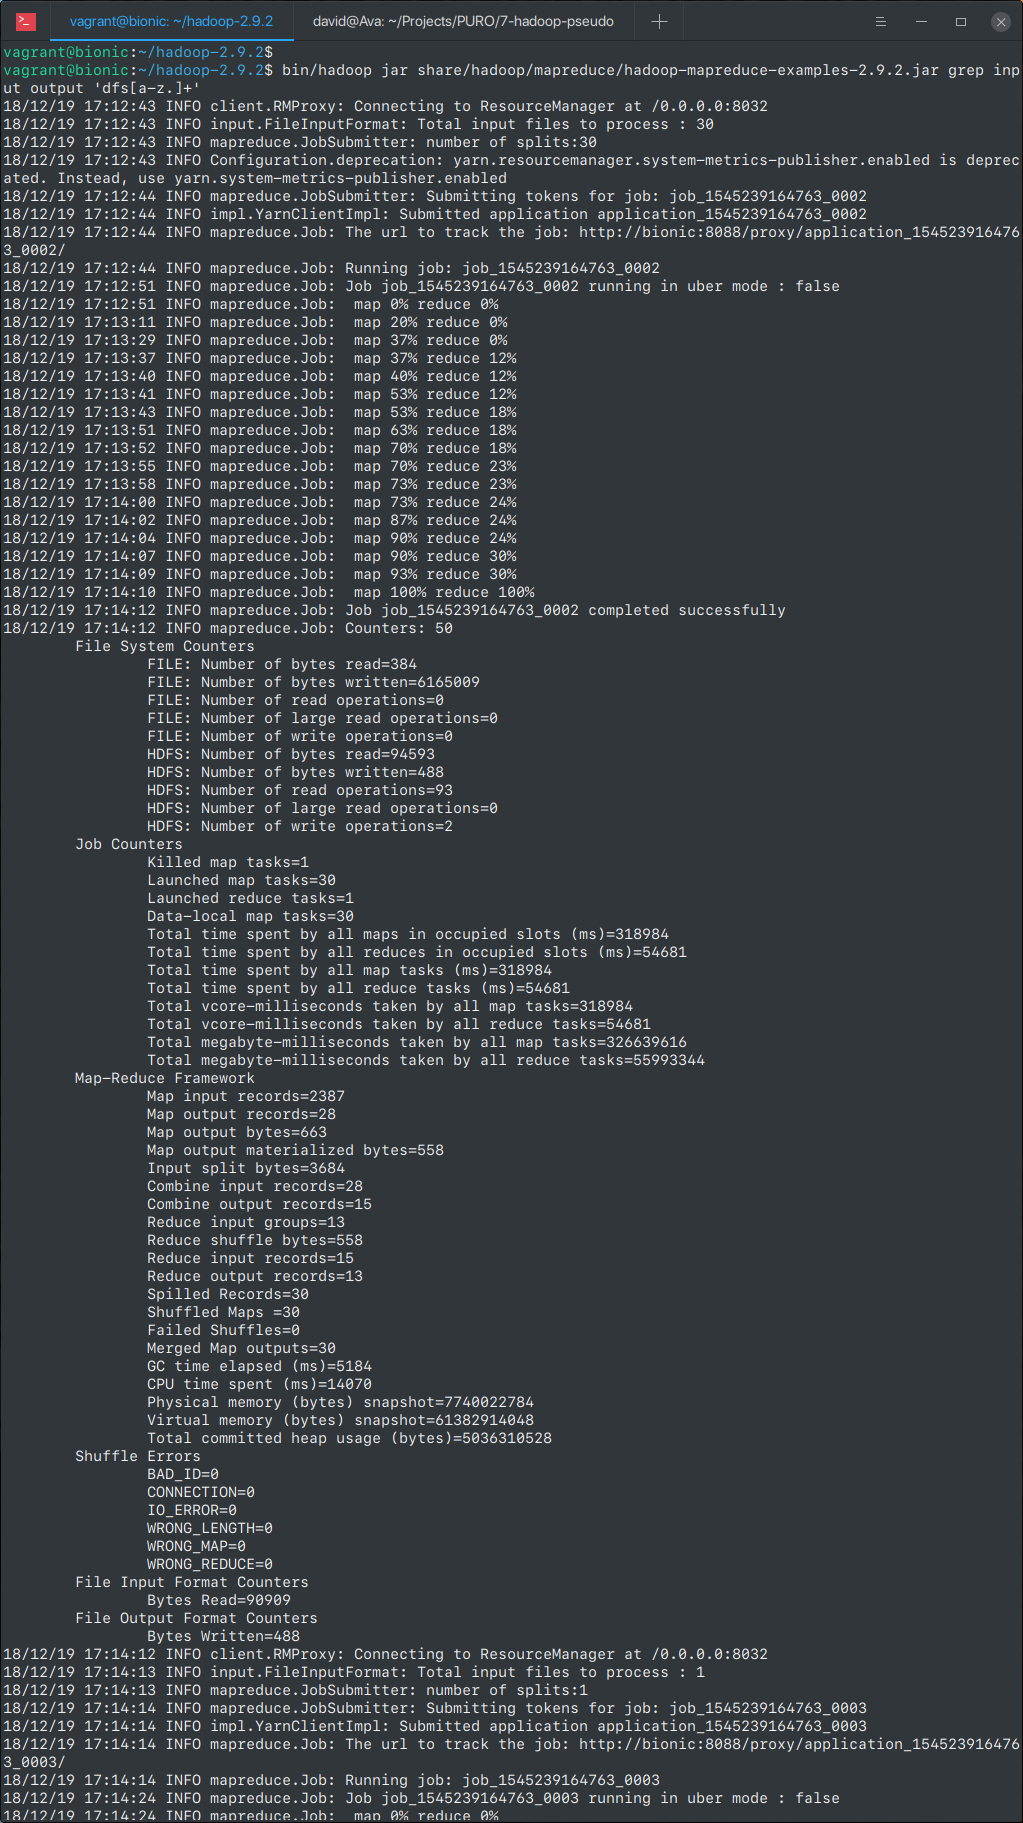
\includegraphics[scale=0.5]{./mapreduce-example.png}
\caption{Primer programa MapReduce, ki teče v sistemu}
\label{example}
\end{center}
\end{figure}


\section{Izjava o izdelavi domače naloge}
Domačo nalogo in pripadajoče programe sem izdelal sam.

\end{document}
